
%----------------------------------------------------------------------------------------
%   PACKAGES & CONFIGURATIONS DU DOCUMENT
%----------------------------------------------------------------------------------------

\documentclass[12pt]{article}
\usepackage[english]{babel}
\usepackage[utf8x]{inputenc}
\usepackage{amsmath}
\usepackage{graphicx}
\usepackage{float}
\usepackage{fancyhdr}
\usepackage[toc,page]{appendix}
\renewcommand\appendixpagename{Appendix}
\renewcommand\appendixtocname{Appendix}
\usepackage[textwidth=17cm,textheight=22cm]{geometry}
\usepackage[colorinlistoftodos]{todonotes}


%----------------------------------------------------------------------------------------
%   HEADER
%----------------------------------------------------------------------------------------
\pagestyle{fancy}
\renewcommand\headrulewidth{1pt}
\fancyhead[L]{RICM4}
\fancyhead[R]{Polytech Grenoble}

\begin{document}

\begin{titlepage}

\newcommand{\HRule}{\rule{\linewidth}{0.2mm}} % Commande définie pour les lignes horizontales (changer l'épaisseur ici)

\center % Centre tout sur la page
 
%----------------------------------------------------------------------------------------
%   TITRES
%----------------------------------------------------------------------------------------

\textsc{\LARGE Polytechnic school of Grenoble-Alpes university}\\[1.0cm] % Nom de l'université
\textsc{\Large RICM4}\\[1.5cm] % Nom de la filière

%----------------------------------------------------------------------------------------
%   TITRE PRINCIPAL
%----------------------------------------------------------------------------------------

\HRule \\[0.5cm]
{ \huge \bfseries Internship report}\\[0.2cm] % Titre du document
\HRule \\[1.5cm]
 
%----------------------------------------------------------------------------------------
%   AUTEUR & TUTEUR
%----------------------------------------------------------------------------------------

\begin{minipage}{0.47\textwidth}
\begin{flushleft} \large

\

\emph{Student :}\\
Julien \textsc{Cordat-Auclair} % Nom
\end{flushleft}
\end{minipage}
~
\begin{minipage}{0.47\textwidth}
\begin{flushright} \large

\

\emph{Supervisor :}\\
Sebastien \textsc{Pittion} % Nom du tuteur
\end{flushright}
\end{minipage}\\[3cm]

%----------------------------------------------------------------------------------------
%   DATE
%----------------------------------------------------------------------------------------

{\large 13 August 2018}\\[4cm] % Date

%----------------------------------------------------------------------------------------
%   LOGO
%----------------------------------------------------------------------------------------


\includegraphics[scale=0.25]{logoUGA.png}\\[1cm] % Logo de l'université
 
%----------------------------------------------------------------------------------------

\vfill % Remplir le reste de la page avec des lignes vides

\end{titlepage}

%----------------------------------------------------------------------------------------
%   PLAN
%----------------------------------------------------------------------------------------

\renewcommand{\contentsname}{Table of content}

\tableofcontents{}

%----------------------------------------------------------------------------------------
%   RAPPORT
%----------------------------------------------------------------------------------------

%   REMERCIEMENTS

\newpage
\section{Acknowledgement}

Before starting this internship report, I would like to thank Mr. Christian Pomot (director of Com\&Net) who accepted to welcome me into his company and who taught me a lot during these 12 weeks by transforming this professional experience into a moment both extremely rewarding and very profitable. He was always available and at listening when I encountered any kind of difficulty, and talking with him allowed me to find a logical solution to each of them.

\

I also thank my supervisor who has regularly assisted me throughout this period with a lot of pedagogy and who has always been available in case of problem. Finally, I would like to thank all the company's employees for their feedback as well as Théo Echevet (student in RICM4) who has helped me several times, without forgetting Mr. Christophe Brouard (researcher at the Laboratoire Informatique of Grenoble) for his help during this project.
\

\

%   INTRODUCTION

\newpage
\section{Introduction}

\subsection{Context}

From May 21 to August 13, I did an internship at \textsc{Com\&Net}. This company specialized in the web allows its customers to develop their websites while optimizing their SEO. During this period, I worked in the company's offices in Grenoble and was accompanied by \textbf{M. Christophe Pomot} (director), two employees, an alternate and \textbf{Théo Echevet}. The company manager provided me clear and precise specifications for the project he had assigned to me, the main requirement being the use of \textbf{M. Christophe Brouard}'s algorithm.

\

\subsection{Mission}

Au cours de ce stage, j'ai dû mettre en place un service permettant de soumettre des recommandations à un utilisateur vis-à-vis du référencement de sa page web pour une requête donnée. L'utilisateur fournit donc l'URL de sa page ainsi que les mots-clés pour lesquels il souhaite que celle-ci soit référencée au mieux et le service doit lui renvoyer un ensemble d'informations l'aidant à atteindre cet objectif. Cette application utilise par ailleurs les algorithmes d'apprentissage machine développés par \textbf{M. Christophe Brouard} appelés \texttt{Echo}. Le projet se distingue donc en trois étapes spécifiques : la collecte des données depuis le web, l'apprentissage machine à partir de celles-ci puis l'affichage des résultats renvoyés par \texttt{Echo}. 

\

Le projet soulève donc des problématiques de back-end et de front-end, établissant ainsi un domaine d'étude à la fois riche et complet, d'autant plus que de multiples langages, frameworks et bibliothèques ont été utilisés : \textsf{Python}, \textsf{PHP}, \textsf{HTML}, \textsf{CSS}, \textsf{JavaScript} ainsi que \textsf{Scrapy} (\textit{scrapy.org}), \textsf{Selenium} (\textit{www.seleniumhq.org}), \textsf{Symfony} (\textit{symfony.com}), \textsf{jQuery} (\textit{jquery.com}) ou encore le moteur de template \textsf{Twig} (\textit{twig.symfony.com}). Par ailleurs, il est important de noter que le service que j'ai mis en place va être utilisé plus tard par la société pour pouvoir faciliter les tâches de référencement, aussi bien pour des clients que des employés spécialisés dans ce domaine qui auront alors un outil de plus à leur disposition pour effectuer ce travail important lorsqu'il s'agit d'établir une stratégie numérique efficace. 

\

Enfin, la performance de ce service doit être optimale pour pouvoir proposer des modifications qui permettront de faire gagner un maximum de places aux sites analysés : il faut en effet noter que seulement les 3 pages les mieux positionnées attirent l'attention des utilisateurs, les autres passant quasiment inaperçues (uniquement 10\% d'attention leur sont accordés). La problématique de référencement est donc primordiale pour toute personne ou société souhaitant se démarquer des autres et l'intérêt qui lui est porté ne peut que s'amplifier au fil du temps.

\

\

\

Voici deux tableaux permettant d'illustrer ce projet ; le premier présente les paramètres entrés par l'utilisateur et le second correspond aux résultats qui lui seront renvoyés :

\

\begin{center}
\begin{tabular}{|c|c|}
\hline
URL de l'utilisateur & http://com-et-net.com \\
\hline
Mots-clés & stratégie numérique grenoble \\
\hline
\end{tabular}

\

\

\begin{tabular}{|c|c|c|}
\hline
\texttt{EchoBT} & référencement\_title, agence\_title, stratégie\_alt, isère\_strong ... \\
\hline
\texttt{EchoPos} & 14 \\
\hline
\texttt{EchoV} & 0.76, 0.63 \\
\hline
\end{tabular}
\end{center}

\

Toutes ces informations seront expliquées plus tard.

\

\subsection{Plan}

Comme énoncé précédemment, trois étapes évidentes se sont dessinées au cours de ce projet et ce seront elles qui formeront le plan de ce rapport. Pour rappel, la première était une étape de web scraping (collecte de données depuis internet), puis venait le machine learning (traitement de ces données) pour enfin laisser place à l'UX Design (optimisation de l'affichage des résultats). Une présentation de l'entreprise dans laquelle j'ai évolué est cependant nécessaire avant de se pencher sur le travail fourni au cours de ces trois derniers mois.


%   COM&NET

\newpage
\section{\textsc{Com\&Net}}

\subsection{Présentation de l'entreprise}

\textsc{Com\&Net} portait le nom de \textsc{Montagne\&Net} jusqu'en 2016. Fondée en 2003 par \textbf{M. Christian Pomot}, cette société est portée sur la création d'outils web spécifiques aux professionnels du tourisme, notamment dans la région du Vercors dans laquelle elle était située auparavant. Aujourd'hui, \textsc{Com\&Net} a renforcé sa présence sur Grenoble en y installant des bureaux, mais elle garde toujours une antenne sur Villard-de-Lans pour pouvoir rester proche de ses anciens clients. C'est en effet dans cette ville que la société a été initialement créée et c'est ici qu'elle a pu se développer.

\

La société accompagne ainsi les projets et la présence sur internet de différentes structures touristiques comme les hôteliers, les stations ou d'autres activités. Ses atouts principaux sont évidemment la maîtrise du domaine informatique mais aussi une excellente approche des différentes problématiques liées au tourisme. Elle propose différents types de services tels que la création de sites internet, l'optimisation du référencement, la promotion de ces derniers ou encore le développement d'applications.

\

\subsection{Développement de sites et d'applications}

L'entreprise maîtrise un large panel de frameworks afin de s'adapter au mieux aux besoins de ses clients. \textsf{Symfony} (un framwork \textsf{PHP} permettant un développement structuré et rapide) et \textsf{Copix} sont les plus utilisés dans le cadre de projets conséquents. \textsf{Thélia} (une solution Open Source apparue en 2006) est aussi un framework que les employés sont capables d'utiliser lorsqu'il s'agit de mettre en place un site d'e-commerce. Ainsi, la société développe de nombreux sites touristiques mais aussi des applications telles que \textsc{GTE} qui permet la traçabilité des explosifs pour les stations de sports d'hiver.

\

En plus de leur création, \textsc{Com\&Net} assure l'hébergement et la maintenance des sites. Les employés restent toujours disponibles auprès des clients pour répondre à la moindre question et sont prêts à régler un quelconque problème à tout moment.

\

\subsection{Stratégie numérique}

\textsc{Com\&Net} est également une entreprise spécialisée en stratégie numérique, c'est-à-dire les différentes méthodes permettant d'optimiser la visibilité des sites internet de ses clients dans les résultats des moteurs de recherche. C'est en partie dans cette optique qu'un partenariat a été mis en place avec l'\textsc{Université Grenoble Alpes} en 2015 pour pouvoir utiliser les algorithmes d'apprentissage machine développés par \textbf{M. Christophe Brouard}.

\

\subsection{Organisation}

\textsc{Com\&Net} est une \textsf{SARL} (Société à Responsabilité Limitée) unipersonnelle, ce qui signifie qu'il y a un unique associé, en l'occurrence \textbf{M. Christian Pomot}. Trois personnes sont employées dans l'entreprise et actuellement accompagnées d'un alternant (cf. \textsl{annexe 1}). Deux secteurs se distinguent clairement au sein de celle-ci : le premier est destiné au développement des sites internet et des applications, le second est dédié à la stratégie numérique et au web-marketing.

\

\subsection{Développement durable}

Pour réduire son empreinte carbone, \textsc{Com\&Net} a choisi de faire héberger ses différents serveurs par \textsc{PHPNET}. Les démarches éco-responsables que cette entreprise grenobloise propose sont les suivantes :
\begin{itemize}
	\item l'utilisation de serveurs SSD offrant une fiabilité optimale et une réduction importante de la consommation électrique (près de 98\% d'énergie en moins que traditionnellement)
	\item le don de l'ancien matériel informatique à l'association \textit{Ulisse Solidura} dans une optique de recyclage grâce à leur atelier nommé \textit{DEEE} (Déchêts d'Équipements Électriques et Électroniques)
	\item  l'utilisation de technologies dites de Free Cooling désignant un refroidissement naturel et permettant donc de refroidir le datacenter de l'entreprise grâce à l'air extérieur si sa température est inférieure à celle de l'intérieur (donc très pratique en hiver)
	\item le raccord des datacenters au réseau électrique de Grenoble \textsc{GEG} (électricité verte)
	\item l'hébergement de serveurs à des associations telles que \textit{Les Jardins de la Solidarité}, un chantier d'insertion mêlant un maraîchage bio, une pépinière et des espaces verts
\end{itemize}

\

De plus, \textsc{Com\&Net} utilise des ordinateurs \textsc{Terra} afin de réduire les consommations électriques dûes au matériel informatique. Ceux-ci sont certifiés par l'\textsc{Energy Star 5.0} et possèdent par conséquent une faible consommation d'énergie. L'entreprise réduit donc la dépense énergétique en plus des émissions de gaz à effet de serre. \textsc{Terra} optimise par ailleurs un peu plus ses ordinateurs au fil du temps (de l'ordre de 35\% de réduction de consommation entre des appareils actuels et des appareils vieux de 3 ans). Les écrans sont également choisis chez cette marque, impliquant une réduction globale de la consommation énergétique encore plus grande.

\

Enfin, il est important de citer que \textbf{M. Christian Pomot} possède une voiture électrique et qu'il est loin d'être insensible au sujet du développement durable. Les stagiaires et alternants qui ont eu l'occasion de travailler dans les bureaux de l'entreprise à Grenoble s'y sont toujours rendu en tramway ou à pied.

%   1ERE PARTIE : WEB SCRAPING

\newpage
\section{Première partie : le web scraping}

\textit{Avant tout développement, un schéma représentant l'architecture générale de cette étape et les liens entre les différents fichiers qui la composent est disponible (cf. \textsl{annexe 2}).}

\subsection{Présentation générale}

La première étape de ce projet portait sur la récupération de données depuis le web. Le stage étant axé autour du thème du machine learning, il paraît en effet essentiel d'être en mesure d'avoir des éléments à fournir à l'algorithme d'apprentissage machine pour qu'il puisse fonctionner. Comme le but du service est d'optimiser le référencement d'une page web, l'idée est de se concentrer sur les données publiques relatives à ce domaine. Cette étape consiste donc à collecter le contenu des balises qui pèsent sur la balance du référencement d'une page web, et ce pour un nombre conséquent de sites affichés suite à une requête Google (cette requête étant choisie par l'utilisateur). On parle alors de SEO On-Site (SEO signifiant Search Engine Optimization, On-Site désignant l’ensemble des actions d’optimisation du référencement qui prennent place au niveau du site web et de ses contenus). Le positionnement du site de l'utilisateur ne peut pas être optimisé de manière optimale grâce à cette méthode puisque le SEO Off-Site (tout ce qui touche à la structure même du site) n'est pas pris en charge par le service. C'est cependant une amélioration que le directeur de Com\&Net envisage fortement dans le cadre de la poursuite de ce projet afin d'obtenir un outil complet mais surtout très performant.

\

Pour réaliser ce travail de web scraping, \textbf{M. Christian Pomot} a tenu à ce que j'utilise le langage \textsf{Python} ainsi que les frameworks \textsf{Selenium} et \textsf{Scrapy} ; le premier permet de simuler un navigateur web ainsi que des interactions ''humaines'' qui vont avec ce dernier (comme un clic de souris ou une touche de clavier pressée) et le second rend possible la création de robots d'indexation capables d'effectuer des tâches de web scraping (ie. récupérer des données \textsf{HTML}). Leur combinaison semble donc parfaitement adaptée au projet.

\


\subsection{Description du travail effectué}

\subsubsection{Récupération des URLs}

Dans un premier temps, j'ai utilisé \textsf{Selenium} pour pouvoir générer une requête Google selon les mots-clés entrés par l'utilisateur. Ces mots-clés, ainsi que l'URL de la page web de ce dernier, sont en fait stockés dans un fichier texte (avec d'autres paramètres) et le moteur de web scraping est capable de les extraire. De cette manière, la récupération des URLs et tout le processus qui suit seront adaptés à la demande de l'utilisateur. Le fichier texte produit est interprété de la manière suivante : 

\begin{center}
 \begin{tabular}{|c|c|c|c|}
\hline
1ère ligne  & URL de l'utilisateur \\
\hline
2ème ligne & nombre de pages à étudier \\
\hline
3ème ligne & degré de pertinence \\
\hline
lignes suivantes & mots-clés \\
\hline
\end{tabular}
\end{center}

\

L'idée est donc de récupérer les URLs présentes sur la page de résultats de la requête utilisateur pour pouvoir en extraire les données qui nous intéressent. Un lien de recherche Google peut s'écrire : \texttt{https://www.google.com/search?q=motclé1+motclé2+motclé3}. Il faut donc simplement changer les mots-clés de ce lien par ceux choisis par l'utilisateur pour pouvoir afficher la page de résultats souhaitée grâce aux fonctions proposées par \textsf{Selenium}. 

\

Par ailleurs, Google affiche par défaut 10 résultats par requête. Cette valeur est modifiable (jusqu'à 100) et il était intéressant de pouvoir faire varier ce nombre qui détermine la quantité d'URLs, donc de données potentielles, à analyser plus tard. J'ai alors rajouté le suffixe \texttt{\&num=100} au lien de la recherche pour pouvoir afficher 100 résultats. Et si l'on souhaite récupérer plus de 100 URLs, alors le script est capable de faire une première requête où il cherche les 100 premières pour ensuite générer une nouvelle requête avec le suffixe \texttt{\&sa=N} indiquant à Google d'afficher la seconde page. Ensuite, il faut répérer dans le code source de la page de résultats les balises qui identifient la présence d'un lien vers une page web. À nouveau, une fonction de\textsf{ Selenium} permet de récupérer le contenu de la balise identifiée. C'est donc ainsi que le script est capable de renvoyer une liste d'URLs classées par position à partir d'un ensemble de mots-clés et d'un nombre de résultats donnés.

\

\subsubsection{Collecte des données HTML}
 
Dans un second temps, \textsf{Scrapy} m'a aidé à sauvegarder les données relatives au SEO pour chacune des URLs trouvées précédemment. Une fois le script faisant intervenir \textsf{Selenium} exécuté, il suffit de fournir la liste d'URLs à \textsf{Scrapy} pour que ce dernier puisse les analyser. J'ai donc spécifié au cours de cette étape les différentes balises importantes vis-à-vis du référencement afin d'en extraire le contenu pour chaque page web précédemment renvoyée. Ainsi, ce sont les balises \textit{title}, \textit{h1}, \textit{h2}, \textit{h3}, \textit{strong}, \textit{a}, \textit{p} ainsi que l'attribut \textit{alt} de la balise \textit{img} et les mots apparaissant dans l'URL du site (après le nom de domaine) qui ont été retenus. D'après \textbf{M. Christian Pomot} ainsi que la majorité des études publiées sur internet, toutes ces valeurs seraient celles qui comptent pour le référencement d'une page web. Google ne confirme cependant pas la véracité de ces suppositions. En revanche, il faut noter que les contenus faisant partie du SEO On-Site changent régulièrement comme en témoigne la balise \textit{keywords} qui était primordiale il y a quelques années mais n'a plus aucun impact aujourd'hui sur le référencement. Et il est très facile de s'adapter à ces variations à travers le script décrit ici puisqu'il suffit de changer manuellement les balises à étudier. 

\

\textsf{Scrapy} permet enfin de renvoyer un fichier \textsf{JSON} contenant toutes les données récupérées : c'est ce fichier qui permettra plus tard de faire le lien avec l'étape d'apprentissage machine. Ce framework est très rapide car il fonctionne de manière asynchrone. C'est cependant un problème ici puisque l'on perd nécessairement la position donnée par l'index de la page analysée dans le tableau d'URLs renvoyé précédemment. J'ai donc dû attribuer une position de manière explicite à chaque page pour pouvoir garder cette information fournie par \textsf{Selenium}.

\

\subsubsection{Lien avec l'apprentissage machine}

Une fois que les données ont été récupérées, l'idée est de pouvoir les transmettre d'une quelconque manière à l'algorithme d'apprentissage machine. Sachant que cette deuxième étape majeure (présentée plus tard) est codée en \textsf{PHP} au sein d'un projet \textsf{Symfony}, il est essentiel de pouvoir fournir depuis \textsf{Python} des données qui seront lisibles non seulement par \textsf{PHP} mais aussi par l'algorithme d'apprentissage machine. Le langage \textsf{PHP} est capable de lire un fichier \textsf{JSON},  donc aucune réelle modification n'est nécessaire sur ce point (mis à part quelques problèmes d'encodage) puisque c'est le format de sortie du script \textsf{Python}. Cependant, l'algorithme développé par M. Christophe Brouard n'est pas capable de lire toute forme de ponctuation, d'accentuation ou encore les espaces doubles, triples, etc. Il est donc nécessaire de faire en sorte qu'il n'y en ait pas et ce le plus tôt possible. Avant de passer à l'étape suivante, un nettoyage complet des données est donc effectué.

%   2EME PARTIE : MACHINE LEARNING

\newpage
\section{Deuxième partie : l'apprentissage machine}

\textit{Avant tout développement, un schéma représentant l'architecture générale de cette étape ainsi que les liens entre les différents fichiers dont elle est composée est disponible (cf. \textsl{annexe 3}).}

\subsection{L'algorithme Echo}

Comme énoncé précedemment, ce stage tourne autour du thème du machine learning puisque la spécification initale la plus importante était l'utilisation de l'algorithme d'apprentissage machine (nommé \texttt{Echo}) développé par \textbf{M. Christophe Brouard}. En réalité, dans le cadre de ce projet, trois algorithmes aux actions précises et découlant de \texttt{Echo} ont été utilisés : \texttt{EchoBT}, \texttt{EchoV} et \texttt{EchoPos}.
\begin{itemize}
	\item \texttt{EchoBT} (\textit{BT} signifiant \textit{best-terms}) permet, étant donnés un ensemble de mots chacun accompagné d'un identifiant et d'un indice de pertinence, de déterminer quels sont les termes qui paraissent être les meilleurs dans une optique d'amélioration du référencement. Compte tenu de ce qui a été fait lors de l'étape précédente, les mots seront les termes contenus dans chaque balise récupérée, l'identifiant correspondra au nom du site associé au mot courant et l'indice de pertinence sera une constante qui déterminera jusqu'à quelle position les sites sont jugés comme étant bien référencés (par exemple, on peut estimer que les 20 sites les mieux référencés sont pertinents, donc ces sites auront un indice de pertinence de 1 et tous les autres auront un indice de pertinence de 2 ce qui correspond à \textit{non pertinent}). Grâce à ces paramètres, l'algorithme sera capable, via des méthodes de machine learning, d'identifier quels sont les termes qui sont importants vis-à-vis du référencement en trouvant ceux qui apparaissent dans les sites pertinents mais pas (ou peu) dans les sites non pertinents. À noter que \texttt{EchoBT} renvoie 30 termes classés par ordre décroissant de score (donc du plus efficace au moins efficace), mais cette valeur peut être modifiée pour en obtenir davantage.
	\item \texttt{EchoV} (\textit{V} signifiant \textit{véracité}) permet avec les mêmes paramètres que ceux de \texttt{EchoBT} de fournir un taux de performance représentant la qualité des résultats renvoyés par \texttt{EchoBT}. En effet, il peut parfois être difficile d'isoler des termes efficaces pour le SEO (par exemple, si tous les termes fournis à \texttt{EchoBT} sont identiques, alors l'algorithme ne sera pas capable de trouver un terme apparaissant dans un des sites pertinents mais qui n'est pas présent dans un site non pertinent) et le taux de performance sera alors très faible. À l'inverse, il peut aussi être aisé de savoir quel terme est \textit{SEO-efficient} (par exemple, si tous les sites jugés pertinents contiennent un terme en commun et que ce terme n'apparaît jamais dans un des sites jugés comme n'étant pas pertinent), amenant ainsi à un taux de performance élevé.
	\item \texttt{EchoPos} (\textit{Pos} signifiant \textit{position}) permet à partir des même paramètres accompagnés en plus du contenu du site de l'utilisateur ainsi que des mots-clés composant la requête Google d'estimer la position de la page fournie pour cette requête. De plus, un taux de confiance est calculé pour savoir s'il faut ou non se fier à se résultat.
\end{itemize}

\

\subsection{Description du travail effectué}

\subsubsection{Architecture du projet Symfony}

C'est à partir de cette étape du projet que le framework \textsf{PHP} \textsf{Symfony} est utilisé. En plus de faire le lien entre la récupération des données et l'affichage des résultats, les algorithmes \texttt{Echo} doivent être appelés au cours de celle-ci. C'est donc probablement la plus importante des trois. \textsf{Symfony} impose une architecture bien particulière et permet de développer en MVC (\textit{Modèle-Vue-Contrôleur}) de manière rapide, propre et efficace. Pour exploiter au mieux ce framework, j'ai dû ordonner mon projet de la manière suivante : 
\begin{itemize}
	\item un premier script (appelé \textit{contrôleur} sous \textsf{Symfony}) permet de récupérer les données : il fait alors le lien avec la première étape. Par ailleurs, il permet également de générer le fichier texte qui contient les paramètres de l'étude à mener et qui est utilisé par le moteur de web scraping.  
	\item un second contrôleur permet d'exécuter les algorithme d'apprentissage machine grâce à ces données : c'est la seconde étape. Celle-ci est primordiale car elle est à l'origine de l'obtention des recommandations vis-à-vis du contenu.
	\item un ensemble de fichiers \textsf{HTML}, \textsf{CSS} et \textsf{JavaScript} permet d'afficher les résultats renvoyés notamment grâce à \textsf{jQuery} ainsi que des appels \textsf{Ajax} successifs (\textsf{Ajax} signifie \textit{Asynchronous JavaScript + XML}  et permet de faire des requête \textsf{HTTP} en \textsf{JavaScript}). C'est la troisième et dernière étape et elle nécessite une réflexion approfondie car il faut afficher beaucoup de données tout en facilitant la lecture faite par l'utilisateur.
\end{itemize}

\

\subsubsection{Transmission des données}

Les algorithmes \texttt{EchoBT}, \texttt{EchoV} et \texttt{EchoPos} utilisés ont besoin de données pour pouvoir fonctionner. Les paramètres fournis par l'utilisateur (mots-clés formant la requête Google et URL de la page) sont écrits dans un fichier texte et accompagnés du nombre de résultats souhaités ainsi que du degré de pertinence. Ce fichier de paramétrage est ensuite transmis au script \textsf{Python} qui va être exécuté. Cependant, une fois les données du scraping récupérées au sein du projet \textsf{Symfony}, un traitement préalable est nécessaire avant d'appeler les algorithmes. En effet, les termes transmis à ces derniers doivent garder l'information liée à la balise à laquelle ils sont associés, sinon des termes de la balise \textit{title} pourraient par exemple être comparés à des termes de la balise \textit{h3} et cela n'aurait pas de sens. C'est pourquoi un suffixe ''\_TITLE'' est ajouté à un terme se trouvant dans une balise \textit{title}, ''\_H3'' pour un terme présent dans une balise \textit{h3}, etc. Ce sera donc sous ce format que seront transmises les données aux algorithmes \texttt{Echo}. De plus, les contenus des pages pertinentes sont dupliqués un certain nombre de fois et en fonction de leur position réelle dans la page des résultats Google afin de leur donner davantage d'importance lors du processus de machine learning.

\

\subsubsection{Appel à Echo et récupération des données}

Chaque algorithme tourne sur un serveur local TCP avec un numéro de port différent. Ainsi, il suffit de se connecter au bon port et de transmettre les informations nécessaires pour pouvoir exécuter l'algorithme qui nous intéresse et récupérer les résultats fournis.

\

Une fois que les algorithmes ont analysé les données, les résultats sont renvoyés au script \textsf{PHP}. Une fonction permet alors de trier les meilleurs termes fournis par \texttt{EchoBT} à la fois par importance de balise (par exemple, la balise \textit{title} est plus importante vis-à-vis du SEO que la balise \textit{strong}) et par score. Cette fonction permet également de limiter le nombre de termes à afficher pour l'utilisateur ; en effet, on ne souhaite par exemple pas avoir 100 termes de la balise \textit{h3}. Ce seront ces données traitées au préalable qui seront affichées plus tard.

%   3EME PARTIE : UX DESIGN

\newpage
\section{Troisième partie : l'affichage des résultats}

\textit{Avant tout développement, des captures d'écran de l'affichage final sont disponibles (cf. \textsl{annexes 4, 5, 6 et 7}).}

\subsection{Présentation générale}

La dernière étape de ce projet est dédiée à l'affichage des résultats précédemment renvoyés par \texttt{Echo}. Elle met en oeuvre des problématiques relevant de l'UX Design (pour \textit{User Experience Design}), domaine de l'informatique qui consiste à concevoir un site web de la meilleure des manières possibles de façon à ce que son utilisation soit optimale. Initialement, les critères de base concernant mon projet et vis-à-vis de l'utilisateur étaient les suivants : 
\begin{itemize}
	\item il doit pouvoir entrer des mots-clés (qui forment la requête Google)
	\item il doit pouvoir entrer une URL (celle de la page qu'il souhaite optimiser)
	\item il doit pouvoir lancer l'étude
	\item il doit pouvoir visualiser les résultats de cette étude
	\item il doit être en mesure de comprendre ces résultats afin de pouvoir en tirer profit
\end{itemize}

\

\subsection{Description du travail effectué}

\subsubsection{Récupération des données}

Avant de vouloir traiter l'affichage des résultats, il faut être capable de se les approprier. Le lien avec l'étape précédente est alors fait en \textsf{jQuery} grâce à des appels \textsf{Ajax} qui permettent notamment de récupérer les informations renvoyées par \texttt{Echo}. Cette méthode permet également d'exécuter chacune des étapes les unes après les autres une fois que l'utilisateur décide de lancer l'étude. Ainsi, il est aisé d'identifier un quelconque problème si jamais une erreur intervient au cours du processus. Enfin, l'utilisation de cette structure assure une vitesse d'exécution optimale et donc un temps d'attente minimal pour l'utilisateur puisque les différentes pages (chargement puis résultats) sont chargées sur place. 

\

\subsubsection{Résultats, affichage et ergonomie}

La troisième étape est axée sur l'optimisation de l'affichage des résultats renvoyés par \texttt{Echo} suite à l'apprentissage fait sur un jeu de données fournit par le script \textsf{Python} ; ceux-ci sont divers et variés et sont composés des éléments suivants :
\begin{itemize}
	\item un entier accompagné d'un pourcentage renvoyé par \texttt{EchoPos} : ils correspondent respectivement à la position estimée de la page de l'utilisateur dans les résultats Google pour la requête donnée et au taux de confiance que l'on peut accorder à ce résultat.
	\item un pourcentage renvoyé par \texttt{EchoV} : il correspond au taux de performance d'\texttt{EchoBT}. Cela permet à l'utilisateur de savoir à quel point il peut avoir confiance dans les résultats fournis par ce dernier.
	\item un ensemble de \textit{n} termes de la forme ''mot1\_BALISE'' où \textit{mot1} correspond à un mot jugé comme étant important vis-à-vis du SEO par \texttt{EchoBT} et \textit{BALISE} désigne la balise dans laquelle se trouve ce terme. L'entier \textit{n} peut être modifié dans le code.
\end{itemize}

\

J'ai décidé de séparer l'affichage en deux parties distinctes : tout en haut de la page, l'utilisateur va voir en premier une section dédiée aux informations générales concerant l'étude qu'il a demandé (cf. annexe). Celle-ci comporte un récapitulatif de sa recherche, la position estimée de sa page, des liens vers les sites les mieux référencés pour la requête donnée sans oublier deux graphes représentant les pourcentages citées précédemment. Des tooltips les accompagnent afin de traduire clairement leur fonction.

\

Ensuite, une deuxième section permet d'afficher les meilleurs termes renvoyés par \texttt{EchoBT}. Chaque terme est rangé dans une sous-partie dédiée à la balise à laquelle il est associé, et tous les termes présents au sein d'une même sous-partie sont classés par odre décroissant de score (un code couleur est utilisé pour en rendre compte). De plus, les sous-parties sont affichées par ordre d'importance de la balise correspondante : les termes de la balise \textit{title} apparaissent en haut car c'est la plus importante vis-à-vis du SEO, mais ceux de l'attribut \textit{alt} appraissent plus bas car celui-ci est jugé comme étant moins efficace.

\

\subsubsection{Fonctionnalités supplémentaires}

Chaque sous-partie est accompagnée d'un champ de texte dans lequel est écrit le contenu de la page à optimiser et qui est associé à la balise qui lui correspond. Ce champ peut être modifié par l'utilisateur : l'idée est de rédiger un nouveau contenu pertinent en utilisant des termes indiqués au-dessus et qui permettent, selon \texttt{Echo}, d'être mieux référencé. Chaque balise a son propre champ qui peut être modifié librement. Une fois les modifications opérées, l'utilisateur gagne alors accès à deux boutons en bas de la page : le premier permet de recalculer la position de la page avec les modifications opérées et le second permet d'exporter les changements sous forme d'un fichier \textsf{JSON}.

%   BILAN

\newpage
\section{Bilan}

\subsection{Analyse du travail réalisé}

Ce projet était complet et a nécessité beaucoup de réflexion vis-à-vis de son organisation. En premier lieu, il a fallu coder un moteur de web scraping en utilisant \textsf{Scrapy} et \textsf{Selenium}. Celui-ci est capable de récupérer les données HTML contenues dans des balises spécifiques des pages web les mieux référencées pour une requête donnée ; il devait surtout permettre de fournir les données nécessaires et nettoyées (accents, ponctuation et espaces inutiles) à \texttt{Echo} pour l'apprentissage machine. Cette étape centrale du stage m'a notamment permis de prendre en main le framework \textsf{PHP Symfony} et j'ai dû, au cours de celle-ci, trouver un moyen de faire le lien avec la précédente tout en conservant l'information liée à la balise associée à chaque terme. Enfin, beaucoup de problématiques liées à l'affichage des résultats et de son ergonomie ont été soulevées, mais cette étape d'UX Design a finalement abouti à quelque chose d'à la fois complet, propre et facile à lire. De plus, c'est lors de celle-ci que j'ai pu découvrir \textsf{jQuery} ainsi que les différents appels \textsf{Ajax}, tout en utilisant les langages web classiques.

\

\subsection{Pour aller plus loin}

L'outil que j'ai pu développer au cours de ce stage n'est pas encore complet et certains points pourraient être améliorés  :
\begin{itemize}
	\item pour l'instant, l'application est dédiée au SEO On-Site (contenu) mais ne tient pas compte du SEO Off-Site (structure). Ainsi, l'optimisation n'est pas totale puisque les modifications proposées portent seulement sur une partie du SEO. De plus, dans l'état actuel de l'application, l'estimation de la position est une estimation basée uniquement sur le contenu et non sur la structure, elle n'est donc pas représentative de la réalité.
	\item il pourrait être intéressant de permettre à l'utilisateur de modifier le nombre de pages à étudier et le degré de pertinence (c'est-à-dire jusqu'à quelle position les sites référencés sont-ils considérés comme pertinents vis-à-vis du SEO). On se rend compte en effet que pour obtenir des recommandations cohérentes (donc un taux de performance très élevé), ces paramètres doivent être adaptés à la requête donnée et ne seront donc jamais identiques. Actuellement, ces valeurs sont fixées dans le code (200 résultats et 30 pertinents) de manière à ce que les résultats renvoyés soient intéressants pour un maximum de requêtes, mais on peut imaginer vouloir laisser l'utilisateur les choisir lui-même. Il lui suffira alors de vérifier que le taux de performance est élevé pour savoir si oui ou non les paramètres qu'il a choisi sont bons. On peut même penser à un système permettant de calculer automatiquement les meilleurs paramètres possibles pour les mots-clés fournis en cherchant à atteindre un taux de performance de 100\%.
	\item certains termes renvoyés par \texttt{EchoBT} sont incohérents (environ 1 sur 5). C'est un phénomène facilement justifiable ; dans le cas de requêtes générales où beaucoup de pages cherchent à se démarquer, les contenus de ces pages seront plus ou moins semblables. Comme \texttt{EchoBT} cherche les termes qui permettent de se démarquer, il ne va pas renvoyer ces mots-clés là mais plutôt des termes qui apparaissent plusieurs fois et dans des pages pertinentes sans qu'ils apparaissent dans les pages non pertinentes. Il s'agit généralement de noms propres et plus précisément de noms de sites.
	
	\underline{Exemple :} on veut optimiser la page de l'entreprise \textsc{Com\&Net} dédiée au web-marketing pour la recherche ''stratégie numérique grenoble''. \texttt{EchoBT} renvoie alors des termes incohérents tels que ''oxiwiz'', ''emalaya'' etc. En fait, on se rend compte en se rendant sur la page de résultats Google que les 50 premiers sites incluent les mots-clés recherchés dans leur titre. Sachant que les 30 premiers sites sont jugés pertinents (et le reste non pertinent), l'algorithme d'apprentissage machine va ignorer ces termes et va renvoyer à la place des mots qui apparaissent plusieurs fois dans les pages pertinentes sans qu'ils n'apparaissent dans les non pertinentes. C'est ainsi que l'on se retrouve avec des résultats incohérents : ''oxiwiz'' et ''emalaya'' sont des noms d'entreprises, et il sont renvoyés car en plus d'être d'être des pages bien référencées, un article apparaissant dans les premiers résultats cite ces derniers. Ce sont donc des termes qui sont répétés dans des pages pertinentes mais pas dans des non pertinentes.
	
	Pour éviter ce genre de problème, j'ai rajouté dans mon code et à l'issue de l'étape de web scraping une fonction permettant de supprimer tout nom propre contenu dans les résultats qui seront plus tard envoyés à \texttt{EchoBT}. Cependant, cela augmente considérablement le temps d'exécution du programme qui est multiplié au moins par 5. Pour gagner du temps tout en assurant la cohérence des résultats, il serait possible d'éxecuter cette étape après avoir reçu les résultats de la part de \texttt{EchoBT}, mais alors des termes seraient éliminés sans être remplacés par d'autres. Actuellement, aucun traitement de ce genre n'est appliqué au niveau de l'outil.
	\item les termes proposés ne contiennent aucun accent car les algorithmes \texttt{Echo} ne peuvent pas les prendre en compte. Il serait donc bon de faire en sorte que ce soit le cas.
	\item enfin, le temps d'exécution du processus (à partir du moment où l'utilisateur clique sur le bouton pour lancer l'étude jusqu'à l'affichage des résultats) mériterait d'être optimisé. Actuellement, celui-ci dure en moyenne une minute mais peut être très variable en fonction de la requête donnée : c'est en réalité l'étape de web scraping qui prend le plus de temps à aboutir et il se trouve que \textsf{Scrapy} a du mal à extraire les données de certaines pages. J'ai donc mis en place un système qui ordonne à \textsf{Scrapy} d'interrompre son action sur une page si celle-ci dure plus de 5 secondes, mais le ralentissement dû à ce léger problème est toujours présent.
\end{itemize}

%   CONCLUSION

\newpage
\section{Conclusion}

Au cours de ce stage, j'ai pu voir pour la première fois comment fonctionnait une entreprise portée sur l'informatique ainsi que les méthodes de travail qui s'y appliquaient. Le projet m'a permis d'améliorer mes compétences dans ce secteur, aussi bien vis-à-vis du back-end que du front-end : j'ai utilisé de nombreux langages et j'ai pris en main de nouveaux frameworks tout en m'intéressant à des nouveaux domaines tels que le web scraping, l'apprentissage machine ou encore l'UX Design. J'ai appris à mettre en place une application du début jusqu'à la fin, chose que je n'avais jamais fait auparavant. Enfin, j'ai découvert une méthode de travail qui me convenait bien puisque j'ai travaillé la plupart du temps seul tout en interagissant régulièrement avec l'extérieur pour obtenir des conseils, des avis ou des solutions.

\

Tous ces paramètres me mènent donc à dire que ces trois derniers mois ont été extrêmement enrichissants, aussi bien sur le plan professionnel par la découverte de différentes façons de travailler et par la complétude du projet réalisé que sur le plan personnel par l'acquisition de nombreuses nouvelles connaissances.

%   RESUMES

\newpage
\section{Résumés}

\subsection{Français}

Le stage effectué sur une période de trois mois était à la fois riche et complet. Il permettait de prendre en main de nombreuses technologies à travers des domaines variés allant du back-end au front-end en passant par du machine learning. Le but du projet proposé était de créer un service permettant à un utilisateur d'optimiser le référencement de sa page web pour une requête donnée. Cette optimisation était notamment permise grâce à des algorithmes d'apprentissage machine dont l'entreprise avait accès. Afin de pouvoir les utiliser, une de mes tâches était de leur fournir des données relatives au contenu d'un certain nombre de pages référencées pour cette requête. Une fois ces données transmises et grâce à un degré de pertinence qui leur était donné, les algorithmes étaient capables de différencier une page bien référencée d'une page mal référencée et donc de filtrer le contenu pour renvoyer les termes à intégrer dans la page de l'utilisateur afin de gagner des places dans les résultats de la recherche. Enfin, un affichage optimisé de ces termes accompagnés d'informations et fonctionnalités supplémentaires a été fait.

\subsection{Anglais}

The internship over a three-month period was both rich and well-furnished. It made it possible to take in hand many technologies through various fields such as the back-end, the front-end and the machine learning. The goal of the suggested project was to create a service allowing a user to optimize the SEO of his web page for a given request. This optimization was made possible by machine learning algorithms that the company had access to. In order to be able to use them, one of my tasks was to provide them data related to the content of a certain number of pages indexed for this request. Once this data was transmitted and thanks to a degree of relevance given, the algorithms were able to differentiate a well indexed page from a poorly indexed one and thus filter the content to return the terms to be integrated in the user's page in order to gain positions in the search results. Finally, an optimized display of these terms with additional information and features has been made.

%----------------------------------------------------------------------------------------
%   ANNEXE
%----------------------------------------------------------------------------------------

\newpage

\begin{appendices}

\

\

\

\

\

\

\begin{figure}[h]
	\centering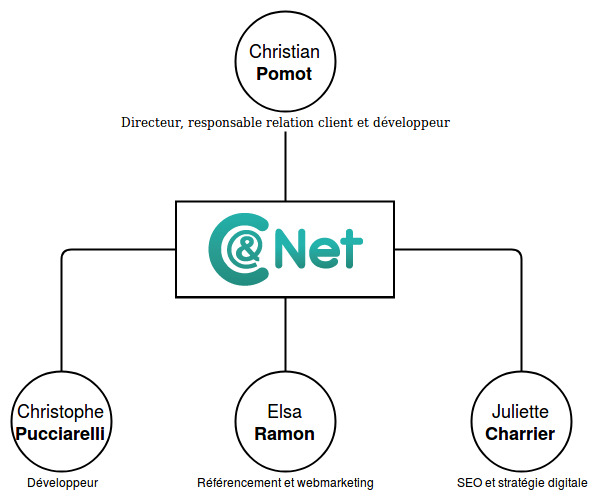
\includegraphics[scale=0.65]{Com&Net.jpg}
	\caption{organisation de l'entreprise Com\&Net}
\end{figure}

\begin{figure}[p]
	\centering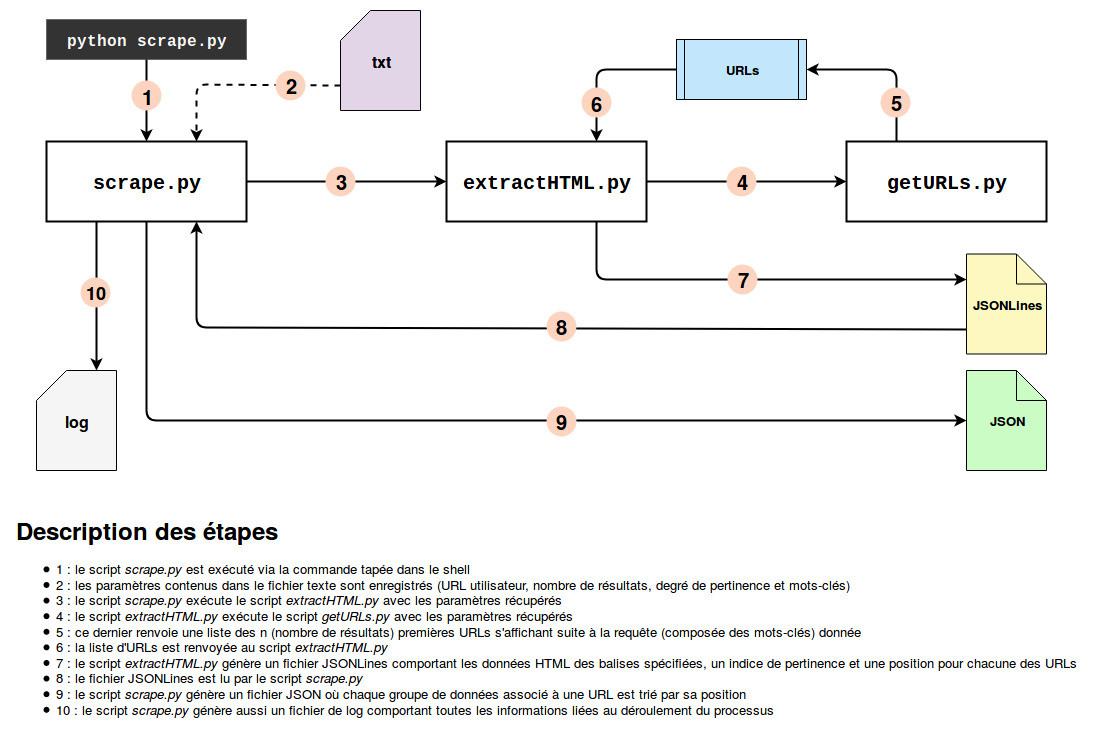
\includegraphics[scale=0.45]{architectureScraping.jpg}
	\caption{représentation schématique de l'architecture du moteur de scraping}
\end{figure}

\begin{figure}[p]
	\centering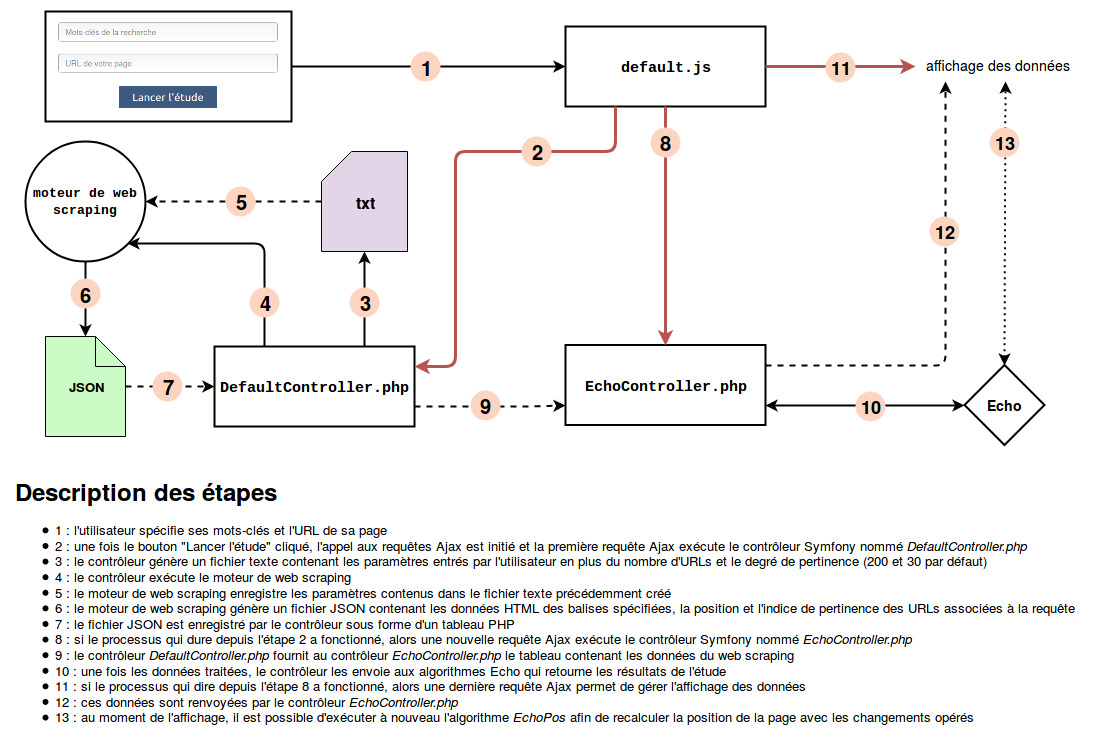
\includegraphics[scale=0.45]{architectureMachineLearning.jpg}
	\caption{représentation schématique de l'architecture du projet Symfony}
\end{figure}

\

\begin{figure}[p]
	\centering
	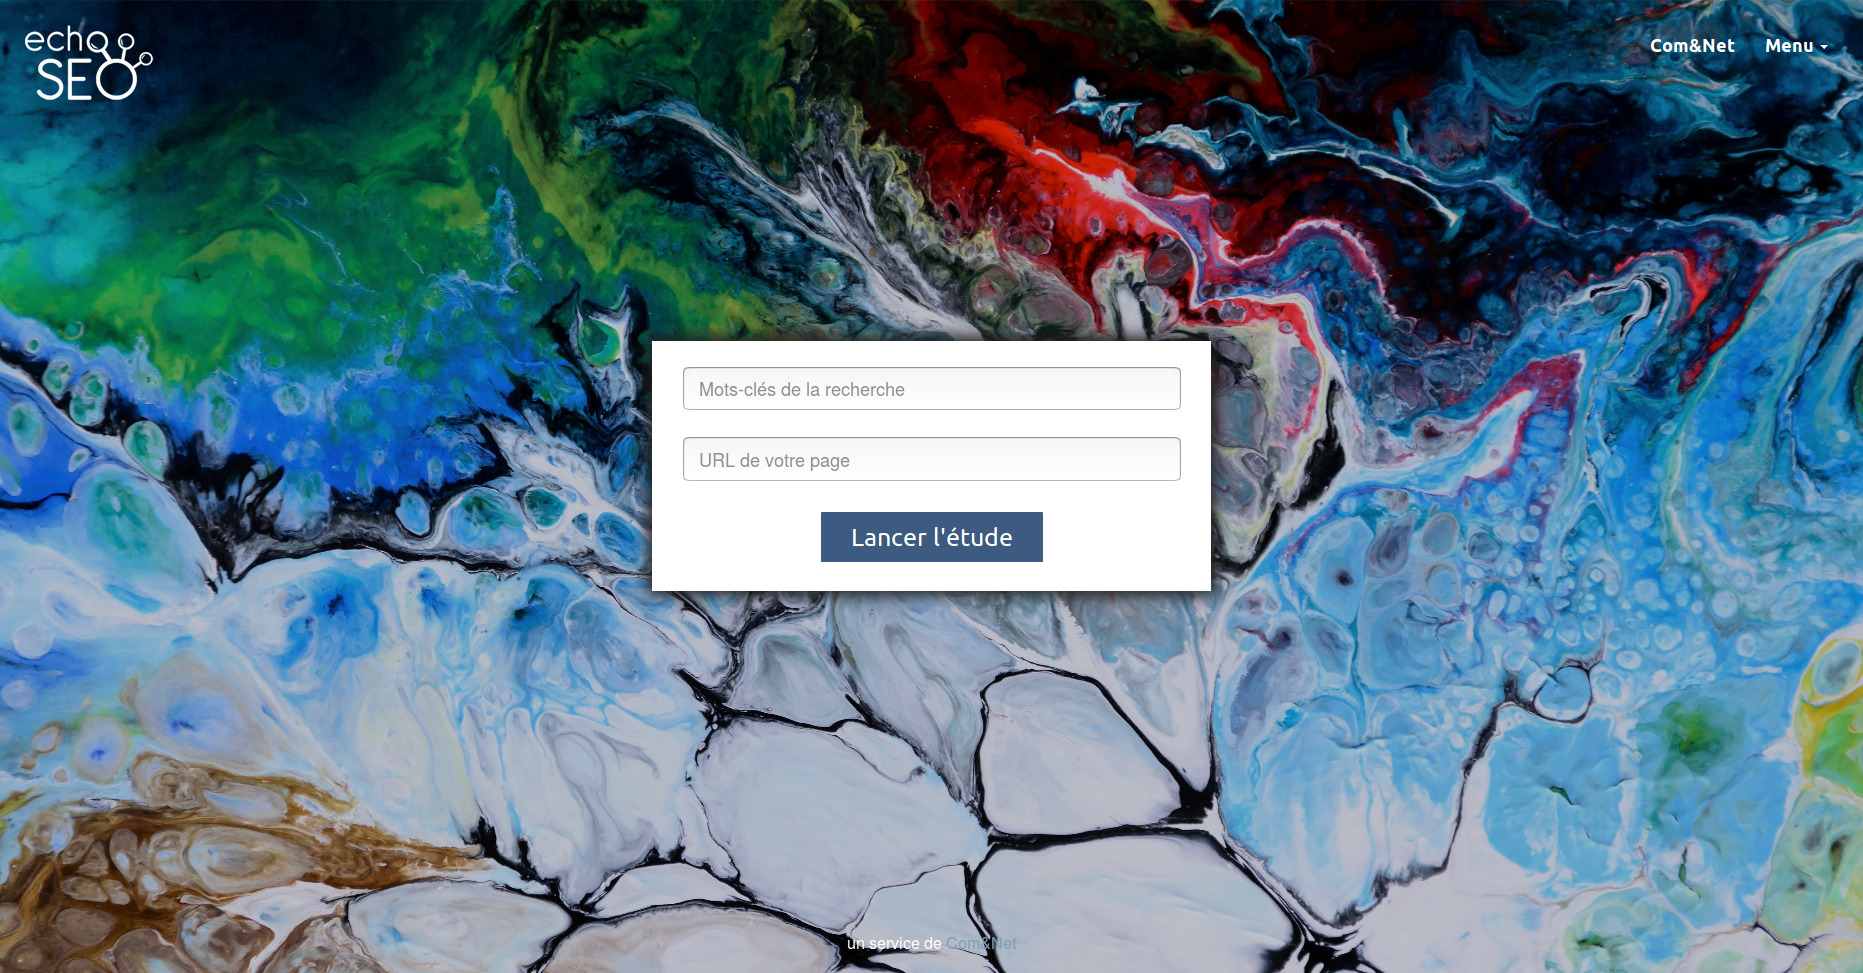
\includegraphics[scale=0.25]{ecranAccueil.jpg}
	\caption{capture d'écran de l'écran d'accueil}
\end{figure}
\begin{figure}[p]
	\centering
	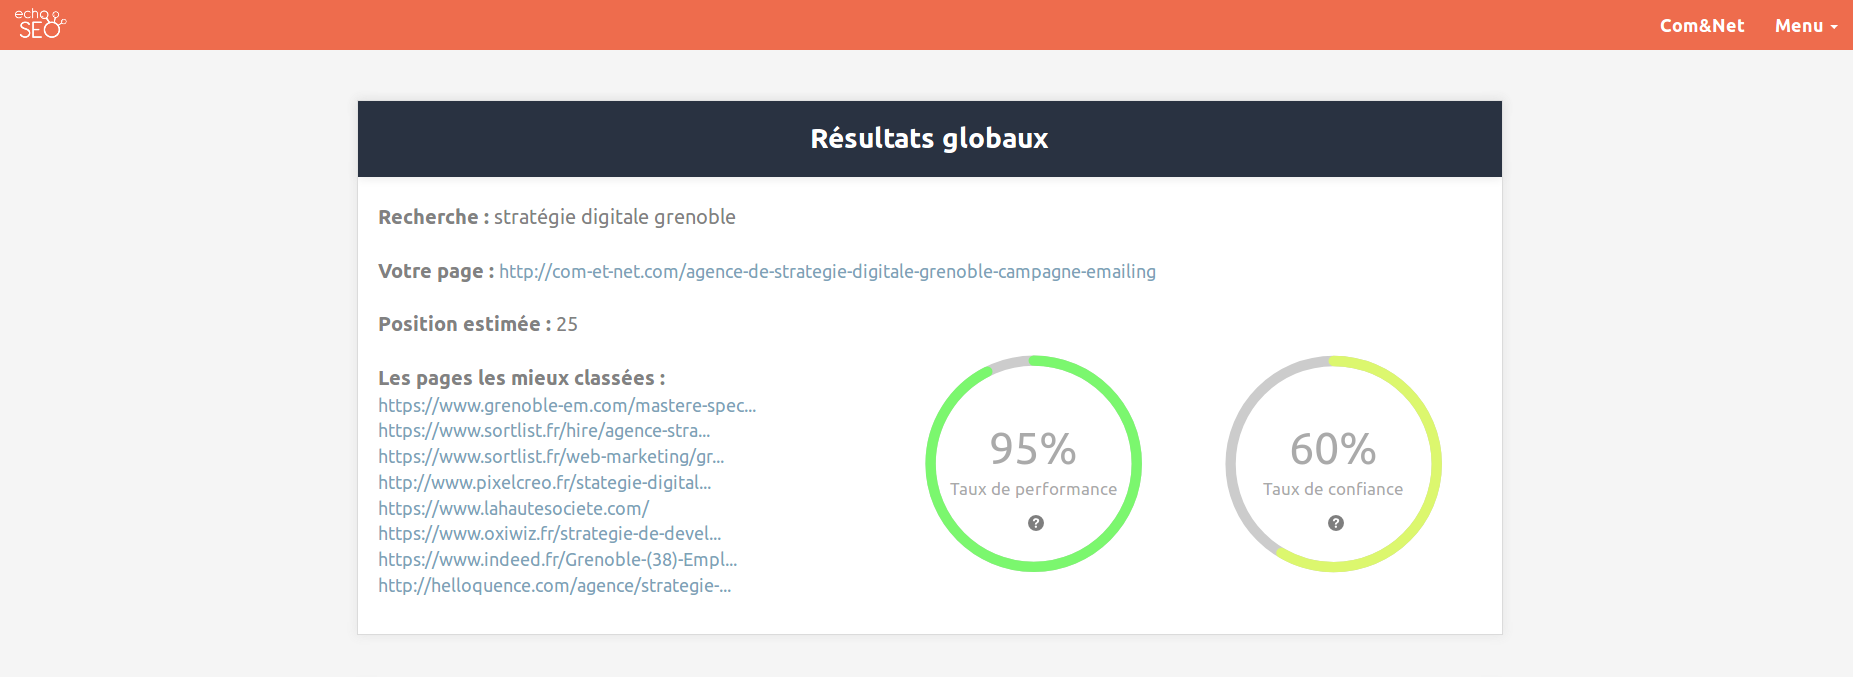
\includegraphics[scale=0.25]{hautDePage.png}
	\caption{capture d'écran du haut de la page des résultats}
\end{figure}
\begin{figure}[p]
	\centering
	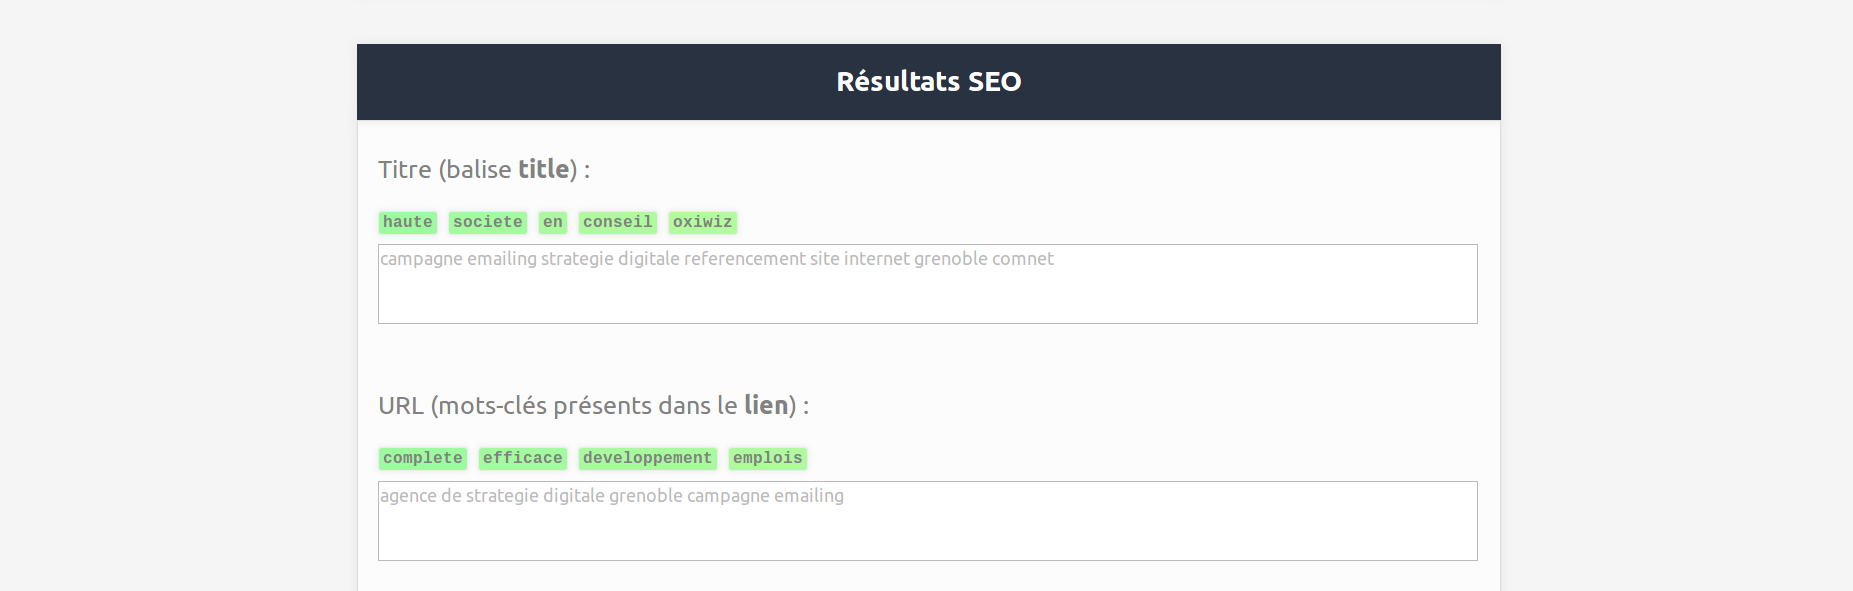
\includegraphics[scale=0.25]{milieuDePage.png}
	\caption{capture d'écran du milieu de la page des résultats}
\end{figure}
\begin{figure}[p]
	\centering
	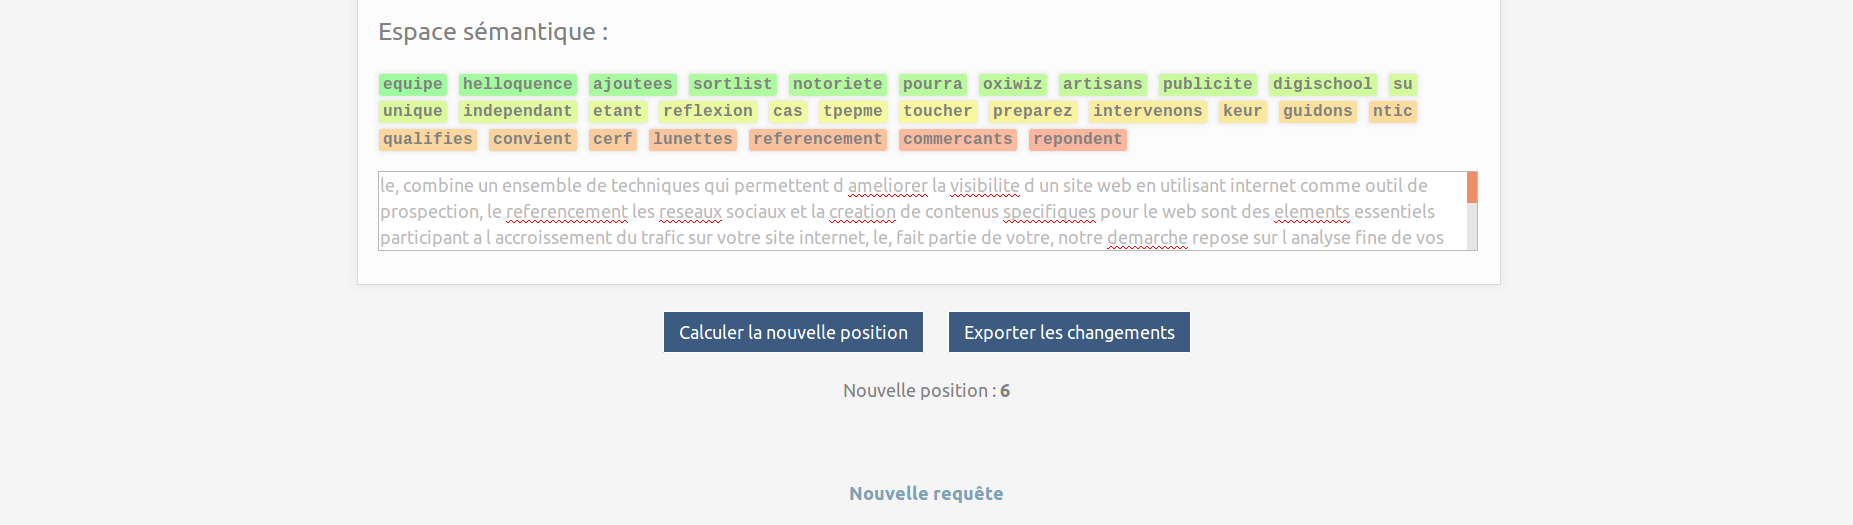
\includegraphics[scale=0.25]{basDePage.png}
	\caption{capture d'écran du bas de la page des résultats}
\end{figure}

\

\newpage
\begin{figure}[p]
	\centering
	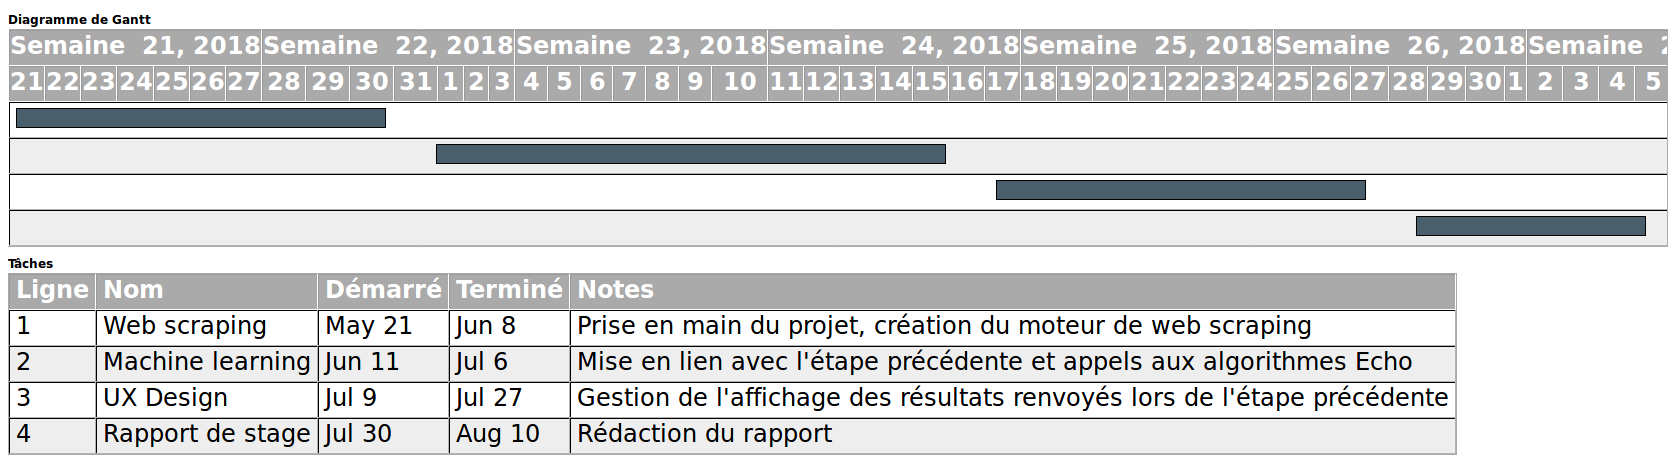
\includegraphics[scale=0.3]{gantt.png}
	\caption{diagramme de Gantt}
\end{figure}

\end{appendices}

\end{document}